\documentclass[11pt]{article}
\usepackage[T1]{fontenc}
\usepackage[utf8]{inputenc}
\usepackage{lmodern}
\usepackage[margin=1in]{geometry}
\usepackage{microtype}
\usepackage{amsmath,amssymb}
\usepackage{graphicx,booktabs,tabularx,array}
\usepackage{enumitem}
\usepackage[numbers,sort&compress]{natbib}
\usepackage{xcolor}
\usepackage{tikz}
\usetikzlibrary{arrows.meta,positioning}
\usepackage[colorlinks=true,linkcolor=blue!50!black,citecolor=blue!50!black,urlcolor=blue!50!black]{hyperref}
\hypersetup{pdftitle={Zyra: A Zero-Shot Robot Manipulation Agent with Sparse Action Programs},pdfauthor={Ziyao Wang},pdfsubject={EZRobot first-generation system technical report draft}}
\usepackage{fancyhdr}
\pagestyle{fancy}
\fancyhf{}
\lhead{\small EZRobot \textbar\ Zyra v1}
\rhead{\small Technical report draft}
\cfoot{\thepage}
\setlength{\headheight}{14pt}
\setlength{\emergencystretch}{2em}
\setlist[itemize]{leftmargin=*,itemsep=2pt,topsep=4pt}
\newcommand{\zyra}{Zyra}
\newcommand{\draftnote}[1]{\par\smallskip\noindent\fcolorbox{orange!40}{orange!6}{\parbox{\dimexpr\linewidth-2\fboxsep-2\fboxrule\relax}{\small\textbf{Draft status.} #1}}\par\smallskip}

\title{\textbf{Zyra: A Zero-Shot Robot Manipulation Agent\\with Sparse Action Programs}\\[0.5em]\large EZRobot First-Generation System Technical Report}
\author{Ziyao Wang\\EZRobot}
\date{October 2026}

\begin{document}
\maketitle
\begin{abstract}
We present \zyra, the first-generation EZRobot manipulation system, built around a general-purpose vision-language model (VLM) rather than a vision-language-action (VLA) policy or a world action model (WAM). Our premise is that robots can acquire broad task competence by combining a foundation model's understanding and program-generation capabilities with measured geometry and closed-loop execution. \zyra\ provides the model with a numbered scene, a table of RGB-D-derived object geometry, and an on-demand measurement interface. The model produces sparse waypoint programs with explicit orientation, gripper, precision, and failure-handling requirements. Execution returns physical feedback for verification and replanning. The system uses no target-task demonstrations or task-specific model training. The current open agent achieves 89/100 successes across four LIBERO suites and 268/300 on six LIBERO-PRO position and task perturbation conditions, with approximately four model calls per episode. Its reported position and task averages are 87.3\% and 91.3\%, compared with published GPT-5.4/Guava-harness averages of 45\% and 44\%; these are cross-system comparisons with different models and evaluation sample sizes. A shared perception and control stack has also been deployed for zero-shot pick-and-place in a real laboratory. This report describes the architecture, available evaluation evidence, deployment experience, and the inference-cost and latency constraints that shape the next generation.
\end{abstract}

\draftnote{Working manuscript based on the implementation snapshot supplied on October 8, 2026. Simulation tables reproduce the recorded v9 evaluations. Full-scale evaluation, current open-agent LIBERO-Plus results, real-robot trial statistics, and the complete author list remain to be incorporated.}

\section{Introduction}
\label{sec:intro}

A robot operating in a laboratory or a home encounters objects, layouts, and instructions that change continually. A request may refer to a new container, require an unfamiliar sequence of familiar motions, or place an object outside the positions represented in training. The central deployment question is whether the system can interpret the new situation and act without another cycle of task-specific data collection and policy training.

VLA policies such as OpenVLA~\citep{kim2024openvla} learn action prediction from robot demonstrations. WAMs such as DreamZero~\citep{ye2026dreamzero} couple action generation with prediction of future visual states. These approaches offer important capabilities, but they also motivate a different architectural question: \emph{can a general-purpose VLM remain the robot's decision maker, with physical action obtained through measured geometry and explicit programs?} Robustness studies on LIBERO-PRO and LIBERO-Plus show why this question matters: high scores in standard environments do not by themselves establish reliability under changed positions, viewpoints, or task conditions~\citep{zhou2025liberopro,fei2025liberoplus}.

Our long-term objective is to establish a VLM-centered alternative to both VLA and WAM architectures for general robot manipulation. We hypothesize that a foundation model's understanding and output capabilities can support adaptation at runtime: interpret an instruction, request the physical quantities needed to act, compose a program, and revise it from execution feedback. The first-generation EZRobot system, \zyra, implements this hypothesis without a VLA action head, a learned action-generating world model, or target-task demonstrations.

The key interface connects reasoning to physical quantities. A VLM can recognize a drawer or a bowl, but an image alone does not provide a reliable metric displacement or grasp center. \zyra\ gives the model measured positions, dimensions, and local surface geometry in the robot base frame. The model uses these measurements to generate a sparse program of end-effector waypoints. Each waypoint specifies motion and execution conditions; a conventional controller performs the high-frequency servoing. The next reasoning round sees the scene before and after execution, fresh geometry, and a structured log describing arrival errors, stalled motion, and finger gaps.

The current system contains two agents sharing the same perception, robot interface, and execution infrastructure. The \emph{open agent} is the main simulation method and synthesizes waypoint programs for grasping, placement, pushing, and articulated manipulation. A frozen \emph{pick-and-place agent} uses typed skill contracts and is the current real-robot deployment path. We distinguish these agents throughout the report so that evidence from one is not attributed to the other.

The present report makes three contributions:
\begin{itemize}
\item A concrete VLM-centered manipulation architecture that connects general-purpose reasoning to RGB-D measurements and sparse programs without target-task policy training.
\item An executable action interface with waypoint-level precision, abort, grip-retention, and end-stop requirements, together with feedback-conditioned verification and recovery.
\item Initial quantitative evidence across standard and perturbed simulation tasks, plus a real-laboratory deployment of the shared stack, and an accounting of the cost and latency challenges of frontier-model inference.
\end{itemize}

The measured results support this architectural direction within the evaluated tabletop tasks. They do not establish unrestricted manipulation, universal replacement of trained policies, or robustness to every form of distribution shift. Our product goal is broader than this first evaluation; the report separates demonstrated capability from that goal.

\paragraph{Meaning of zero-shot.}
We use \emph{zero-shot} to mean that no demonstrations from the evaluated target tasks are used for model training and no target-task model fine-tuning is performed. \zyra\ does use a pretrained VLM, engineered perception and control, robot calibration, and written manipulation guidance. Foundation-model pretraining data are outside our control. System development on benchmark scenes is disclosed separately from task-specific model training.

\section{System Architecture}
\label{sec:method}

\subsection{Reason, Measure, Program, and Execute}
At reasoning round $r$, the system observes RGB-D data and robot self-state, denoted $o_r$. A geometric perception module produces an object table $G_r$. The VLM receives the instruction $\ell$, the image, $G_r$, selected manipulation knowledge $K_r$, and execution history $H_r$. Its output is either a measurement request, a waypoint program, or a task verdict:
\begin{equation}
 y_r = F_\theta(\ell,o_r,G_r,K_r,H_r).
\end{equation}
The parameters $\theta$ remain fixed. Measurement requests are answered from the current calibrated depth observation, after which the model is queried again. A valid program is executed by the robot backend. Physical execution updates the scene and yields a log $L_r$, which is included in the next round. The main configuration permits up to three execution rounds and a final review round. Each round can contain multiple model requests, so a round is not equivalent to one model call.

\begin{figure}[t]
\centering
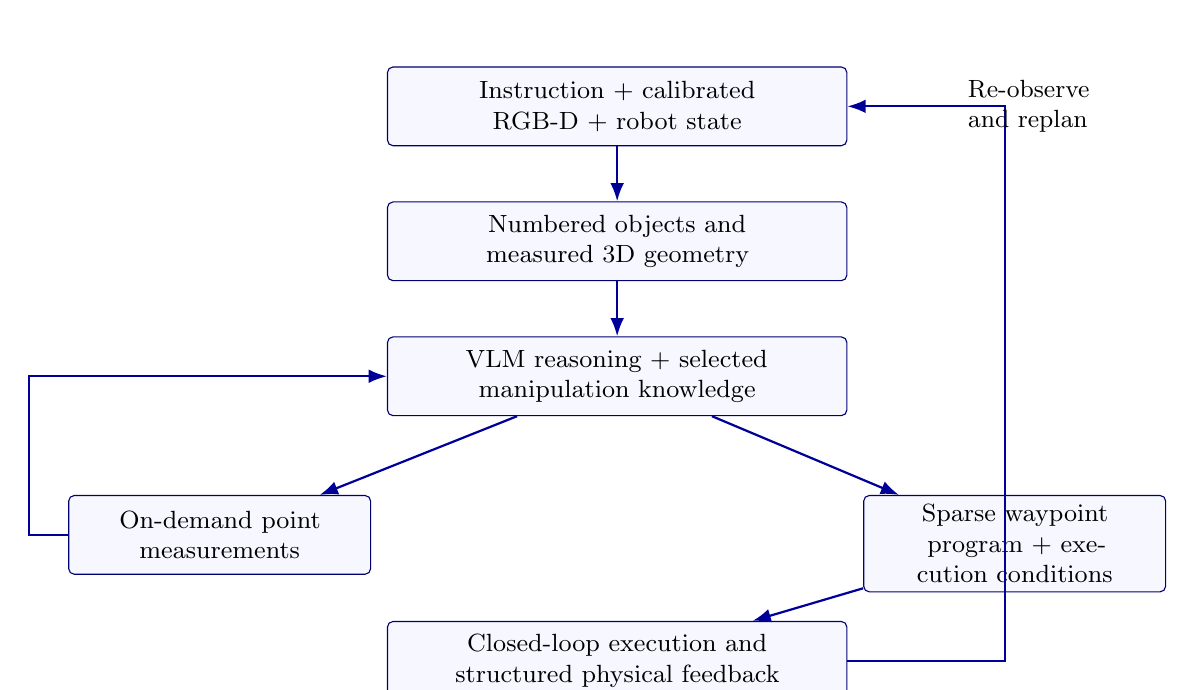
\begin{tikzpicture}[node distance=7mm and 10mm,>=Latex,
 box/.style={draw=blue!45!black,fill=blue!3,rounded corners=2pt,align=center,text width=5.6cm,minimum height=10mm,font=\small},
 arrow/.style={->,thick,draw=blue!60!black}]
\node[box] (obs) {Instruction + calibrated RGB-D + robot state};
\node[box,below=of obs] (geo) {Numbered objects and measured 3D geometry};
\node[box,below=of geo] (vlm) {VLM reasoning + selected manipulation knowledge};
\node[box,below left=10mm and 2mm of vlm,text width=3.6cm] (measure) {On-demand point measurements};
\node[box,below right=10mm and 2mm of vlm,text width=3.6cm] (program) {Sparse waypoint program + execution conditions};
\node[box,below=26mm of vlm] (exec) {Closed-loop execution and structured physical feedback};
\draw[arrow] (obs)--(geo);
\draw[arrow] (geo)--(vlm);
\draw[arrow] (vlm)--(measure);
\draw[arrow] (measure.west) -- ++(-0.5,0) |- (vlm.west);
\draw[arrow] (vlm)--(program);
\draw[arrow] (program)--(exec);
\draw[arrow] (exec.east) -- ++(2.0,0) |- node[pos=.65,right,font=\small,align=left] {Re-observe\\and replan} (obs.east);
\end{tikzpicture}
\caption{The main open-agent loop. Geometry is obtained through perception and measurement; the VLM chooses and parameterizes the operation; the backend handles servoing. Benchmark goal labels are used only by the evaluator.}
\label{fig:architecture}
\end{figure}

\subsection{Measured Scene Geometry}
For a depth pixel $(u,v)$ with depth $d$ and calibrated intrinsic matrix $K$, a surface point is mapped into the robot base frame by
\begin{equation}
 \begin{bmatrix}p_{\mathrm{base}}\\1\end{bmatrix}
 = T_{\mathrm{base}\leftarrow\mathrm{camera}}
 \begin{bmatrix}dK^{-1}[u,v,1]^\top\\1\end{bmatrix}.
\end{equation}
Depth components above an estimated support plane produce a class-agnostic object table. Entries include visible bounds, top height and center, and narrow/wide planar axes and widths. Objects are numbered on the image; the numbers carry no semantic identity, and the VLM associates entries with the instruction. The implementation limits the table to 14 entries. Thin surfaces and large fixtures may be absent, so the table is complemented by requested measurements.

Single-view geometry can systematically underestimate an object's center. A camera observes the near side of a can or bowl, whose surface centroid differs from the object's physical axis. For vertically oriented round objects, v9 fits a shared planar center across thin height slices using robust least squares: points within a slice should have approximately equal radial distance from that center. The inferred axis completes the round body's center and bounds. Regions with consistent axes can be merged, preventing the walls of one bowl from appearing as unrelated objects. This is a geometric prior about shape, not a semantic object detector or an oracle object pose.

For parts outside the object table, the VLM marks image pixels. A measurement returns a robust local 3D point, height above the table, a fitted surface normal where supported, and local principal directions and extents. The implementation permits up to eight requested points per call. The model computes action targets from these quantities. Target positions include planned offsets and displacements, so they are \emph{derived from} measurements rather than all being directly observed surface coordinates. Measurement provenance is encouraged through a textual calculation field; the current implementation does not formally prove that every generated coordinate follows from the supplied measurements.

\subsection{Sparse Programs and Execution Conditions}
A program contains an ordered list of end-effector waypoints. Each waypoint specifies a metric position $p_i$, approach direction $a_i$, closing axis $c_i$, gripper state after arrival, and execution conditions. The orientation is constructed from the approach and closing directions. Validation rejects malformed or non-finite vectors, degenerate orientations, nominal positions outside configured workspace bounds, and targets outside a configured reach approximation. The main configuration allows at most 24 waypoints.

\begin{table}[t]
\centering\small
\begin{tabularx}{\linewidth}{@{}lX@{}}
\toprule
Field & Execution meaning \\
\midrule
\texttt{precision} & Fine arrival: 4 mm position and 0.08 rad rotation; coarse transit: 2 cm and 0.2 rad. \\
\texttt{if\_blocked} & Abort subsequent waypoints when arrival fails, or continue when contact is intended. \\
\texttt{must\_hold} & Require an occupied finger gap after closing; abort later motion if the gap indicates grip loss. \\
\texttt{until\_blocked} & Extend the move up to 10 cm beyond its nominal point and report stalled motion and measured travel. \\
\bottomrule
\end{tabularx}
\caption{Waypoint-level requirements in the current open-agent executor. These conditions make intent and failures inspectable; they do not constitute a formal collision-free motion guarantee.}
\label{tab:contract}
\end{table}

The controller follows Cartesian targets while maintaining the current gripper state, then applies the requested gripper transition. Motion is monitored in short windows. Lack of positional and rotational progress ends a segment early and is recorded as a stall. Finger gap provides a coarse indication of whether something is held. Neither stall nor finger gap is a direct force/contact measurement: a stall can reflect an obstacle, a joint constraint, or an intended end stop, and a nonzero gap does not guarantee a stable grasp.

Sparse programs separate model reasoning frequency from control frequency. A single program may contain a grasp, transport, placement, and retreat, or approximate an articulated motion with several short segments. The system logs each segment and returns the arm toward its start pose so the fixed camera can observe the outcome. Returning home also consumes control budget and can change the final task state; the evaluation therefore records both any-step and final-state success.

\subsection{Feedback, Knowledge, and Recovery}
Before the initial program, a triage call identifies likely difficulties and selects short manipulation notes. The library covers articulated parts, containers, grip security, flat objects, hand clearance, blocked moves, pushing, reach posture, spatial relations, surface support, and multi-step tasks. These notes describe reusable physical considerations. They are engineered priors and are included in the system's zero-shot definition.

Later rounds receive the earlier image, current image and geometry, the previous program, and waypoint feedback. The agent may request fresh measurements, choose a different contact or approach, or complete the remaining subtask. Contact-related failures can additionally retrieve blocked-motion guidance. Task completion is the model's own verdict, conditioned on available measurements and logs. It is not an independently verified certificate of success; comparison against the external evaluator exposes its errors.

\subsection{Shared Stack and Real-Robot Path}
The earlier pick-and-place agent asks the VLM for semantic objects, 2D target prompts, and typed skill calls. Geometric grounding compiles these into grasp and placement poses. Active wrist observations address uncertain side views; obstacle relocation and retries are available. This agent uses fixed skill contracts rather than freely generated waypoint programs. It is retained as the current hardware path and as a separately versioned reference system.

The robot interface exposes calibrated images, depth, robot self-state, TCP servoing, and gripper actuation. Benchmark construction, oracle segmentation, and goal predicates are confined to the evaluation harness. Source-isolation tests prohibit the method package from importing the benchmark package. This is an engineering separation, not a security sandbox: the simulation backend necessarily accesses the simulator for sensor rendering, robot state, and calibration, but the agent's observation interface contains no benchmark object identities or goal labels.

\section{Simulation Evaluation}
\label{sec:eval}

\subsection{Protocol and Evidence Scope}
The main results concern open-agent v9 with Claude Opus through the Claude Code CLI. The system receives no target-task demonstrations and performs no task-specific model training. LIBERO~\citep{liu2023libero} supplies the standard manipulation suites, and LIBERO-PRO~\citep{zhou2025liberopro} supplies position and task perturbations. We use the suite-specific post-settling control budgets: 220 steps for Spatial, 280 for Object, 300 for Goal, and 520 for Long. Perturbed tasks inherit the corresponding suite budget.

\emph{Standard success} means the LIBERO BDDL goal predicate is reached at some recorded control step within budget. \emph{Final-state success} means it still holds when the agent finishes. The agent does not receive this predicate. Its own completion claim is tracked separately. Infrastructure failures are retried by the harness and are not counted as manipulation failures; consequently the task success rates are conditional on completed evaluation episodes rather than a measure of service availability.

The standard-suite sample contains 25 episodes per suite: initial states 15--16 for every task, and state 17 for tasks 0--4. Thus it spans 40 tasks with two or three initial states per task. It is a development-linked evaluation sample, not a newly frozen independent test: these episodes were also used to compare v8 and v9 after failure analysis. LIBERO-PRO uses tasks 0--9 and initial states 0--4 for each condition, yielding 50 episodes per condition. Full-protocol evaluations are in progress. Results in this draft reproduce the recorded runs; raw episode archives are not included with the manuscript.

\subsection{Four Standard LIBERO Suites}
\begin{table}[t]
\centering
\begin{tabular}{@{}lrrr@{}}
\toprule
Suite & Successes & Trials & Success rate \\
\midrule
Spatial & 22 & 25 & 88\% \\
Object & 25 & 25 & 100\% \\
Goal & 20 & 25 & 80\% \\
Long & 22 & 25 & 88\% \\
\midrule
Overall & 89 & 100 & \textbf{89\%} \\
\bottomrule
\end{tabular}
\caption{Open-agent v9 on the available standard LIBERO sample. Final-state success is 87/100 overall. The subset is smaller than the common 50-trials-per-task evaluation and should not be treated as a full leaderboard submission.}
\label{tab:libero}
\end{table}

Table~\ref{tab:libero} shows competence across grasping, spatial relations, articulated tasks, and long-horizon compositions with one agent configuration. The 89\% aggregate is evidence of broad capability across this sample. It does not demonstrate superiority over the highest standard-suite VLA results, and the Object score alone is not sufficient to characterize general manipulation.

The recorded v8-to-v9 comparison improves standard success from 76/100 to 89/100 and final-state success from 71/100 to 87/100. Seventeen episodes change from failure to success and four in the opposite direction. However, v9 changes both geometric perception and execution behavior, and the served model for v8 was not recorded. We therefore present this as a system-version comparison, not a controlled estimate of the causal effect of one component.

\subsection{LIBERO-PRO: Changed Positions and Tasks}
\begin{table}[t]
\centering\small
\setlength{\tabcolsep}{5pt}
\begin{tabular}{@{}llrrrrr@{}}
\toprule
Suite & Perturbation & \zyra & GPT-5.4 & Guava-4B & $\pi_{0.5}$ & CaP-Agent0 \\
\midrule
Object & Position & \textbf{98} & 61 & 60 & 17 & 22 \\
Object & Task & \textbf{100} & 57 & 60 & 1 & 18 \\
Goal & Position & \textbf{84} & 44 & 39 & 38 & 26 \\
Goal & Task & \textbf{82} & 47 & 38 & 0 & 17 \\
Spatial & Position & \textbf{80} & 29 & 25 & 20 & 12 \\
Spatial & Task & \textbf{92} & 26 & 26 & 1 & 14 \\
\midrule
Average & Position & \textbf{87.3} & 45 & 41 & 25 & 20 \\
Average & Task & \textbf{91.3} & 44 & 41 & 1 & 16 \\
\bottomrule
\end{tabular}
\caption{Success rates (\%) on six LIBERO-PRO conditions. \zyra\ uses 50 episodes per condition. All other columns reproduce Table 3 of Guava~\citep{liu2026guava}; its $\pi_{0.5}$ and CaP-Agent0 values are in turn attributed to CaP-X~\citep{fu2026capx}. Published averages are rounded as in their source. Baselines were not rerun in our environment.}
\label{tab:pro}
\end{table}

\zyra\ succeeds in 131/150 position-perturbation episodes and 137/150 task-perturbation episodes, for 268/300 overall. The same prompt and agent serve all six conditions. This provides initial evidence that changing where objects start or what the instruction requires can be handled through runtime interpretation and geometric grounding, without adapting model weights.

The position and task averages exceed the published GPT-5.4/Guava-harness averages by approximately 42 and 47 percentage points, respectively. The differences are large across all six reported conditions. They are \emph{cross-system observations}: \zyra\ uses Claude Opus, the baselines use other models and interfaces, evaluation sample sizes differ, and observation resolutions and depth/geometry access must be aligned for an interface-only comparison. The current results cannot isolate how much of the gap comes from the VLM, metric grounding, program interface, or recovery logic.

Under the stricter final-state reading, successes are 49, 50, 41, 34, 40, and 46 in the row order of Table~\ref{tab:pro}, totaling 260/300. The largest standard-to-final difference occurs in Goal/Task. Reporting both readings reveals cases where the goal is attained temporarily and later lost; it avoids equating transient attainment with a stable completed task.

\subsection{Earlier Pick-and-Place Results and LIBERO-Plus}
The separately frozen pick-and-place route achieved 99/100 within-budget successes on a held-out LIBERO-Object sample. Its initial-position LIBERO-PRO run achieved 45/50, and its LIBERO-Plus robot-initial-state sample achieved 85/100. The latter covers 100 Object-suite variants stratified across five difficulty levels, with 19/20, 20/20, 17/20, 17/20, and 12/20 successes. These results belong to the earlier agent and are not included in the v9 main tables.

LIBERO-Plus~\citep{fei2025liberoplus} enables a wider investigation of layout, camera, robot-state, language, lighting, texture, and sensor changes. The supplied snapshot describes current open-agent evaluation as in progress. We will incorporate its complete task manifest and quantitative results when available. The earlier Object/robot-state subset cannot be compared directly with published all-suite averages or used to claim robustness across every perturbation family.

\subsection{Failure Analysis}
The recorded standard-suite v9 failures include unsuccessful stove-knob manipulation, failed placement into the microwave, difficulty extracting a bowl from the top drawer, plate pushing, and a drawer-plus-bowl task. Three episodes claim completion despite failing the evaluator: a drawer opens insufficiently, a bowl lies just outside the plate-center tolerance, and a pudding box misses a benchmark-defined spatial region.

Two recurring mechanisms explain these failures. First, physical execution can fail because the whole hand contacts nearby geometry, a grip slips, or the selected approach is ineffective. Second, the measured or inferred scene quantities may not support sufficiently precise verification. Single-view surface geometry is incomplete, and a physical object center need not equal the benchmark's model origin. The current executor can detect stalled motion but cannot reliably distinguish a desired end stop from an unintended jam. A retry then consumes the remaining control budget. These failure modes motivate better geometry and physical feedback rather than instruction changes alone.

\section{Real-Laboratory Deployment}
\label{sec:real}

The shared stack has been deployed on a UFACTORY 850 arm with an xArm parallel-jaw gripper, a fixed RealSense D435, and a wrist-mounted D435. A Jetson host runs the perception and robot interface; the current planner is accessed through Claude Code. The system has executed zero-shot pick-and-place in the laboratory, demonstrating a hardware deployment of the shared architecture.

The hardware route in the supplied configuration is the pick-and-place agent. Its simulation logic is retained while the backend changes to real sensing and controller-managed Cartesian motion. Camera-to-base transforms are obtained through markerless scene alignment or board-based hand-eye calibration. The documented markerless check used four matched objects and obtained 3.1 mm alignment RMS, with a separate fingertip consistency check within approximately 1 mm horizontally and 6 mm vertically. These are calibration diagnostics, not manipulation success statistics.

Real depth is noisier and incomplete. The side geometry image is pooled to $640\times360$ from $1280\times720$ using temporal and block medians. Wrist observations are always used to confirm the grasp because side views underestimate visible object widths and wrist depth is cleaner at the shorter working distance. The backend uses a fingertip TCP convention and converts controller flange poses accordingly.

\paragraph{Current evidence.}
The report includes qualitative deployment capability; it does not yet contain a counted real-robot evaluation or a claim of open-agent articulated manipulation on hardware. The completed task list, number of attempts, success definitions, interventions, and video examples should be added from the actual run records. Camera calibration and configuration changes must be disclosed alongside the absence of task demonstrations or model fine-tuning.

\paragraph{Execution boundary.}
Motion must be enabled explicitly. The real backend rejects targets outside its configured workspace, preserves controller-side constraints, and latches nonrecoverable controller errors. The application can request operator confirmation. These mechanisms support supervised deployment but do not guarantee collision-free trajectories or force-safe contact. In particular, transferring the open agent's simulation stall logic to hardware requires validating how controller timeouts and contact faults are represented.

\section{Product Performance and Next-Generation Priorities}
\label{sec:discussion}

\subsection{Inference Cost and Latency}
The present product bottleneck is frontier-model inference. Sparse planning reduces the frequency of large-model decisions relative to per-control-step reasoning, but each serial call can still dominate the time a user waits. Triage, requested measurements, program repair, and outcome review all contribute. Claude Code additionally mediates requests through a command-line process and image-reading tools. Its reported usage is an API-equivalent estimate, not necessarily the cash cost of a subscription-backed deployment.

\begin{table}[t]
\centering
\begin{tabular}{@{}lrr@{}}
\toprule
Recorded run & Calls/episode & USD-equivalent/episode \\
\midrule
Open-agent v9, standard LIBERO sample & 4.1 & 0.74 \\
Open-agent v9, six LIBERO-PRO conditions & 3.5--5 & 0.67 \\
\bottomrule
\end{tabular}
\caption{Available model-use accounting from the recorded evaluations. The LIBERO-PRO call count is a reported range across conditions. These costs describe the evaluated backend, not a deployment price guarantee.}
\label{tab:cost}
\end{table}

For an episode with model requests $j=1,\ldots,N$, a useful product accounting separates
\begin{equation}
 T_{\mathrm{total}} = T_{\mathrm{capture/geometry}} + \sum_{j=1}^{N}T_j^{\mathrm{request}} + T_{\mathrm{motion}} + T_{\mathrm{other}}.
\end{equation}
End-to-end latency should include failed attempts and reviews, and be summarized by median and tail percentiles. Cost per successful task should be computed as total cost across all attempted episodes divided by the number of successful episodes; averaging costs only over successes hides expenditure on failures. The available v9 notes do not provide a complete latency distribution, so this draft makes no quantitative v9 speed claim.

\subsection{Optimization Without Changing the Core Route}
Our next-generation priorities preserve the measured-program interface. First, direct model transport can separate model latency from CLI and tool overhead; its quality must be checked on the same frozen episodes rather than assumed. Second, simple tasks may bypass a separate triage request, and measurement requests can be batched. Third, prompts and structured outputs can be shortened while retaining the fields needed for physical execution and verification. Fourth, a lower-cost model can handle straightforward decisions with escalation on uncertainty or failure. These are planned interventions, not measured improvements in this report.

Stable prompts and reusable geometry can be cached only when their assumptions remain valid. Scene measurements become stale after motion, and command reuse across changed objects or layouts requires re-grounding. Any optimization should be evaluated against success, false completion claims, total latency, and cost per successful task. An agent that answers faster but repeats failed grasps can increase deployment cost.

\subsection{Generalization as a Testable Product Property}
The product vision is a robot that adapts to new requests through understanding and interaction. Evidence should therefore be organized by what changes: object instances, layouts, instructions, task compositions, environments, and robot embodiments. Standard-suite performance measures competence on available tasks; perturbation performance tests selected forms of robustness. Hardware deployment tests a different sensing and execution stack. None alone proves arbitrary generalization.

The current evaluation does not cover high-frequency dynamic manipulation, deformables, dexterous in-hand skills, or arbitrary unstructured contact. The program executor relies on engineered geometry and controller behavior, and the open agent currently reasons from a fixed side view. A development-linked benchmark sample also cannot replace a newly frozen independent evaluation. Full-scale held-out runs and controlled interface ablations are the next evidence priorities. Our long-term claim is an architectural hypothesis about the route to general robotics; the present empirical claim is strong zero-shot performance within the recorded tasks and perturbations.

\section{Related Work}

\paragraph{Learned action and world-action models.}
OpenVLA learns an action policy from robot demonstrations and supports adaptation through fine-tuning~\citep{kim2024openvla}. DreamZero explores a WAM based on a pretrained video diffusion backbone with joint future-state and action prediction~\citep{ye2026dreamzero}. These works study routes to generalization through learned action generation. \zyra\ instead keeps a general-purpose VLM as the decision maker and derives execution targets through explicit measurements and programs. We do not evaluate a WAM baseline in this report, so the architectural comparison is not a measured performance ranking against WAMs.

\paragraph{Programs and embodied harnesses.}
Code as Policies established language-model-generated programs for embodied control, including waypoint-based behavior~\citep{liang2022code}. CaP-X studies coding agents across perception/control abstraction levels and test-time interaction~\citep{fu2026capx}. Guava provides a manipulation harness and distills frontier-model interaction behavior into a compact agent~\citep{liu2026guava}. These works are close precedents. Our distinguishing emphasis is the integration of measured object geometry and requested local measurements with freely composed waypoint programs carrying execution conditions. The main experimental question is how well this concrete interface supports zero-shot task and position changes. The report does not claim to be the first use of VLMs, tool feedback, or code generation in robotics.

\paragraph{Generalization benchmarks.}
LIBERO provides manipulation tasks for studying knowledge transfer~\citep{liu2023libero}. LIBERO-PRO and LIBERO-Plus extend evaluation to changed task conditions and systematic perturbations~\citep{zhou2025liberopro,fei2025liberoplus}. They motivate separating standard-task scores from evidence of robustness. \zyra\ currently reports position and task perturbations for the open agent, while wider open-agent LIBERO-Plus evaluation remains in progress.

\section{Conclusion}

\zyra\ implements a VLM-centered route to robot manipulation: interpret the request, measure the scene, generate a sparse physical program, and revise from execution feedback. The first-generation open agent reaches 89\% success on the recorded four-suite LIBERO sample and 89.3\% across six LIBERO-PRO conditions without target-task demonstrations or model training. A shared stack has also executed zero-shot pick-and-place in a real laboratory. These results motivate developing general robot competence through foundation-model reasoning and measured action interfaces. The next generation focuses on preserving that competence while reducing model waiting time and cost, expanding independent evaluation, and extending the open-agent route on hardware.

\bibliographystyle{plainnat}
\bibliography{references}
\appendix
\section{Implementation and Reproduction Details}

The open agent resides in \texttt{src/spar/open}: \texttt{agent.py} implements reasoning rounds, \texttt{measure.py} implements object geometry and point measurement, and \texttt{program.py} implements program validation and execution. The fixed-skill route resides in \texttt{src/spar/agent}. Shared perception, planning, skills, and backends reside in their corresponding packages. The evaluation harness lives in \texttt{spar\_bench}; the hardware cell lives in \texttt{spar\_real}.

The main open-agent configuration uses at most three execution rounds, 24 waypoints, and eight requested points per call. Geometry uses a $256\times256$ simulation depth image; the model sees a separate 1024-pixel render of the same camera. The served model recorded for the standard v9 evaluation is \texttt{claude-opus-5-5}; the configuration itself uses the \texttt{opus} alias. For the LIBERO-PRO run, the report notes a Claude Opus backend but does not enumerate exact served identifiers. Exact served-model identifiers should be recovered from per-call records for every final evaluation.

The standard v9 result is associated with implementation revision \texttt{600fe26}; the LIBERO-PRO result with \texttt{01215c2}. The supplied source snapshot is \texttt{3b298125fab3f9db4234648853329459010d1b3a}. These identifiers are provenance recorded by the source archive and experiment notes; they are not claims that all tables were generated from the supplied snapshot.

\begin{table}[h]
\centering\small
\begin{tabularx}{\linewidth}{@{}lXX@{}}
\toprule
Evidence item & Current draft includes & Required update \\
\midrule
Standard LIBERO & v9 subset; any-step and final-state totals & Full protocol, episode archive, frozen test manifest \\
LIBERO-PRO & Six v9 conditions; published baseline table & Full-size runs, input/model alignment, raw records \\
LIBERO-Plus & Earlier Object/robot-state subset & Current open-agent results by perturbation family \\
Real robot & Hardware route and qualitative execution & Tasks, counted trials, interventions, videos \\
Efficiency & Calls and API-equivalent cost & Latency percentiles, actual charges, per-success cost \\
Mechanisms & Version comparison and implementation & Controlled geometry/feedback/knowledge ablations \\
\bottomrule
\end{tabularx}
\caption{Evidence status for completing the first public report. Pending measurements are not substituted with estimated scores.}
\end{table}


\end{document}
